\section{手法}
\subsection{Mapleとの通信手法}
Mapleは一般的に,グラフや数式の綺麗な出力や,数式の入力を初心者が直感的におこなえるようにJavaで作られたGUIを使って実行する.それとは別にcommand lineで実行される計算エンジン部が用意されている.そこで,開発するRubyライブラリでは,このエンジンに直接働きかけて操作する.Rubyで外部コマンドを実行するgem libraryのsystemuを使って,出力を得るようにしている.Ruby codeで要求コードを受け取った場合,そのコードをtmp.mwに書き込む.それをMapleで実行し,結果をテキストファイルで受けとることで出力を得る.

\subsection{Maple関数の類型化}
今回,数多く存在するMapleの数学関数の中から整数論と行列に関するものを選抜し実装した.

\begin{figure}[htbp]\begin{center}
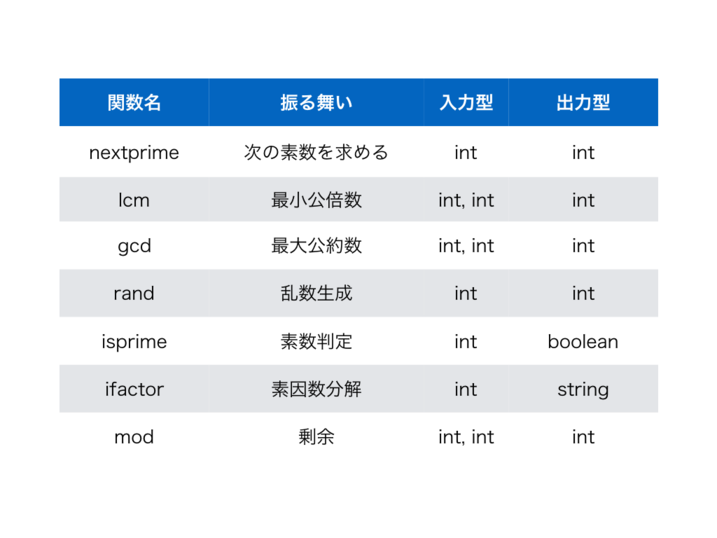
\includegraphics[width=6cm,bb=0 0 442 500]{../figs/./mapleruby_eringi.001.png}
\caption{実装した整数論に関する関数の役割と入出力}
\label{default}\end{center}\end{figure}
\begin{figure}[htbp]\begin{center}
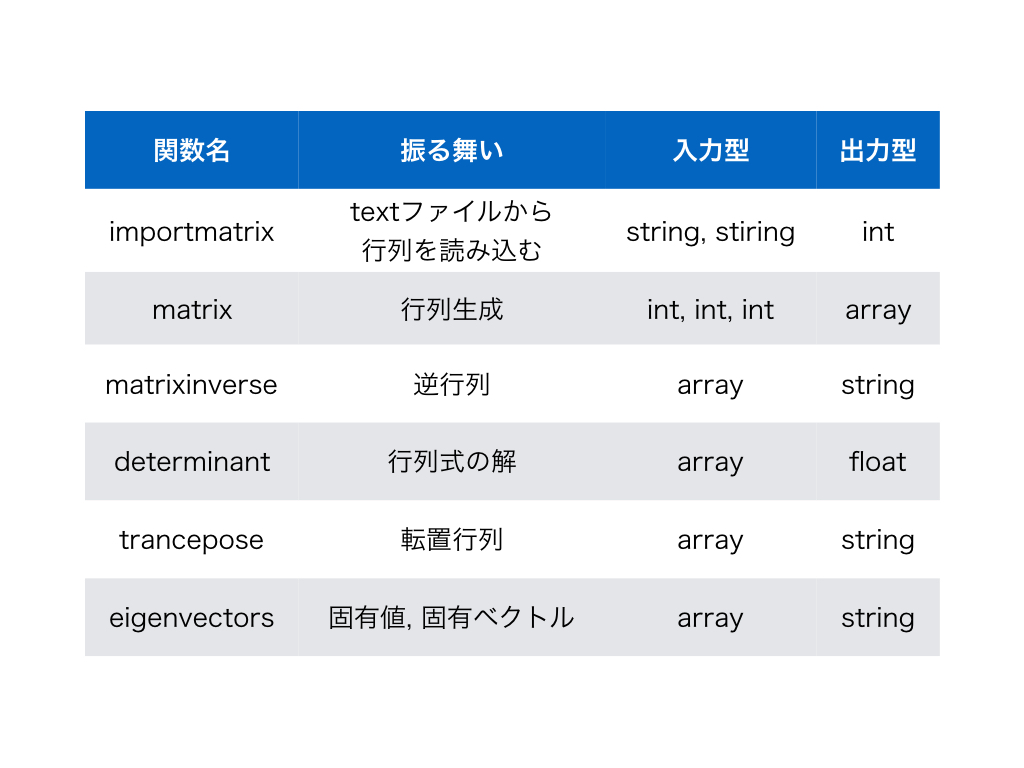
\includegraphics[width=6cm,bb=0 0 442 500]{../figs/./mapleruby_eringi.002.png}
\caption{実装した行列に関する関数の役割と入出力}
\label{default}\end{center}\end{figure}
\subsection{出力の切り替え}
Mapleから受け取ったままの出力は,値の前にスペースがたくさん入っていることや,出力が String 型であることから,その数値を使って計算をするようにプログラミングしていた場合に支障をきたす.このため,関数ごとに正しい型で出力できるようにwrapperを作る.
例えば,int 型で出力が欲しいものはexecをexec\_iから呼び出すことで対応する.このようにbooleanやfloatといった出力型に応じて,exec\_b,exec\_fのように関数を増やしていく.

